\documentclass[12pt, a4paper]{article}
\usepackage[utf8]{inputenc}
\usepackage[fontset=none]{ctex}
\setCJKmainfont[BoldFont=PingFang SC, ItalicFont=Kaiti SC]{Songti SC}
\setCJKsansfont{PingFang SC}
\setCJKmonofont{STSong}
\usepackage{geometry}
\usepackage{amsmath, amssymb, amsfonts} % for math
\usepackage{graphicx}
\usepackage{float}
\usepackage{hyperref}
\usepackage{booktabs} % for better tables
\usepackage{caption}

\geometry{left=2.5cm, right=2.5cm, top=2.5cm, bottom=2.5cm}

\title{\textbf{\Large 基于红外与可见光图像融合的全天候目标检测研究}}
\author{学号:25121360 \quad 姓名:陈艺彬}
\date{\today}

\begin{document}

\maketitle

\begin{abstract}
本报告主要解决复杂光照下的目标检测问题。因为单一传感器在黑夜或强光下容易失效,所以我们设计了一个结合红外和可见光图像的新框架。我们没有简单叠加图像,而是利用红外图像发现目标,并用可见光图像确认细节。我们在特征融合层引入了坐标注意力机制(Coordinate Attention),并采用端到端的训练策略。结果表明,这种方法不仅效果好,而且显著提高了检测精度。
\end{abstract}

\section{项目背景}

\subsection{任务概述}
在计算感知领域,单一传感器有很大局限。可见光相机在暗光下看不清,红外相机没有纹理。所以,我们需要将两者结合,这正是本项目——**可见光与红外(VI-IR)图像融合**要做的事。我们通过处理这两种信息,来获得更准确的场景描述。

\subsection{现有挑战}
虽然有很多算法,但是在实际应用中面临挑战:
\begin{enumerate}
    \item \textbf{位置与含义不匹配}:现有方法虽然通过生成让图像变好看,但是丢失了小目标的空间信息。所以检测器很难画出精准的框。
    \item \textbf{策略缺陷}:大多数算法只追求好看,而不考虑机器能不能检测到。如果丢失了边缘信息,那么融合就是无效的。
\end{enumerate}

\subsection{本文贡献}
针对这些问题,我们提出了一种检测驱动的框架。主要贡献包括:
\begin{enumerate}
    \item \textbf{引入简单的形状规则}:我们针对道路场景,首次在融合层引入了 **Spatial-Coordinate Attention Fusion Module (S-CAFM)**。车道线是水平的,行人是垂直的。S-CAFM 机制利用这一规则,分别在水平和垂直方向上处理特征,这一机制充当了回归任务的“空间标尺”,解决了卷积网络下采样导致的位置信息丢失问题。
    \item \textbf{端到端的联合训练策略}:传统的融合与检测往往是分阶段进行的,通过“接力”的方式传递信息。而我们采用了**端到端联合训练**,通过链式法则,检测网络(YOLOv8 Head)的边界框回归损失(Bounding Box Regression Loss)被转化为对前段融合生成器 $G$ 的梯度更新。这种机制迫使融合层不再关注那些无关紧要的背景纹理,而是全力保留对检测任务至关重要的边缘和轮廓信息:
    \begin{equation}
        \nabla_{\Theta_{Fusion}} = \frac{\partial \mathcal{L}_{Det}}{\partial \mathbf{I}_{Fused}} \cdot \frac{\partial \mathbf{I}_{Fused}}{\partial \Theta_{Fusion}}
    \end{equation}
\end{enumerate}

\textbf{预期结果}:在MSRS数据集上验证所提方法的有效性,实现比单一模态更高的平均精度(mAP),并保持较低的推理延迟。

\section{相关工作}

\subsection{深度学习与图像融合}
近年来,基于深度学习的红外与可见光图像融合方法取得了显著进展,主要分为基于自编码器(Auto-Encoder, AE)、基于生成对抗网络(GAN)以及基于Transformer的方法。
\begin{enumerate}
    \item \textbf{基于AE的方法}:经典算法如 DenseFuse \cite{li2018densefuse} 利用致密连接网络提取特征,并通过L1范数进行重构,虽然保留了较好的纹理,但在融合层设计上较为简单,难以处理复杂光照。
    \item \textbf{基于GAN的方法}:FusionGAN \cite{ma2019fusiongan} 首次将生成对抗网络引入融合任务,通过对抗训练迫使融合图像保留红外热辐射信息,但由于缺乏对可见光梯度的强约束,往往导致纹理细节丢失。
    \item \textbf{基于Transformer的方法}:针对CNN感受野受限的问题,SwinFusion \cite{ma2022swinfusion} 引入了Swin Transformer来捕捉长距离依赖关系,显著提升了融合图像的全局一致性。
\end{enumerate}

\subsection{检测驱动的图像融合}
传统的融合算法仅追求视觉效果(Visual Quality),而忽略了融合图像对下游任务(如目标检测)的友好性。因此,近年来涌现了一批**任务驱动**的融合算法:
\begin{itemize}
    \item \textbf{SeAFusion} \cite{tang2022seafusion} 提出了一种语义感知的实时融合架构,通过引入高层语义损失(Semantic Loss)来引导融合网络保留关键目标特征。
    \item \textbf{PIAFusion} \cite{tang2022piafusion} 进一步考虑了光照变化,设计了基于光照感知的渐进式融合策略,在不同光照条件下均表现出色。
    \item \textbf{TarDAL} \cite{liu2022target} 即本项目选用的Baseline,采用了双对抗学习机制,分别对红外目标和可见光背景进行对抗判别,确保了检测目标的显著性。
    \item \textbf{SuperFusion} \cite{tang2022superfusion} 则将图像配准与融合整合到一个统一框架中,解决了实际场景中非配准图像的融合难题。
\end{itemize}

如图 \ref{fig:tardal_perf} 所示,TarDAL 在保证高精度的同时具有极低的推理延迟,这也是我们选择其作为 Baseline 的主要原因。

\begin{figure}[H]
    \centering
    \includegraphics[width=0.95\textwidth]{images/tardal_performance.png}
    \caption{主流融合算法的性能对比及 $M^3FD$ 数据集统计 (来源: CVPR 2022 \cite{liu2022target})。左图显示 TarDAL (红色) 在效率与精度上取得了最佳平衡。}
    \label{fig:tardal_perf}
\end{figure}

尽管上述方法在检测任务上取得了突破,但在处理**道路场景特有的几何结构**(如车道线、直立行人)时,仍缺乏针对性的空间位置建模能力,这正是本文引入 Coordinate Attention 的动机所在。

\section{方法描述}

\subsection{问题定义}
我们将红外与可见光图像融合任务定义为一个**检测驱动的特征协同重构问题 (Detection-driven Feature Synergistic Reconstruction)**。

形式化地,给定融合网络 $G$ 和检测网络 $D_{det}$,我们的联合优化目标是:
\begin{equation}
    \min_{\Theta_G, \Theta_D} \mathcal{L}_{detect}(D_{det}(G(I_{ir}, I_{vi})), Y_{gt}) + \lambda \mathcal{L}_{fusion}(G(I_{ir}, I_{vi}), I_{ir}, I_{vi})
\end{equation}
其中 $\Theta_G$ 为融合网络的参数,$\Theta_D$ 为检测网络的参数。此公式体现了一个多目标联合优化算子:$\mathcal{L}_{detect}$ 保证语义正确性,而 $\mathcal{L}_{fusion}$ 保证视觉分布的真实性。

\subsection{系统架构概览}
本项目提出的级联式融合检测系统构建在 **TarDAL** \cite{liu2022target} 的基础之上。如图 \ref{fig:arch_detail} 所示,我们在特征提取与重构之间嵌入了核心的**坐标注意力(S-CAFM)模块**。

图 \ref{fig:arch_detail} 展示了**具体的网络架构**。特征提取部分采用类似 DenseNet 的密集连接块,核心的融合层嵌入了我们设计的坐标注意力(S-CAFM)模块。检测部分采用了 **YOLOv8 Head** 来从融合特征中提取语义信息。

\textbf{训练策略:端到端检测驱动 (End-to-End Detection-Driven)}。
尽管系统在推理时是级联结构,但在训练阶段,我们构建了一个完整的闭环。如图 \ref{fig:arch_detail} 所示,检测网络 $D_{det}$ 的预测误差(包含 Bounding Box 回归损失和类别损失)通过反向传播算法直接作用于融合网络 $G$ 的参数更新。
\begin{itemize}
    \item \textbf{前向传播}:融合图像 $I_f$ 输入 YOLOv8 产生检测结果。
    \item \textbf{反向传播}:$\nabla_{\Theta_G} \mathcal{L}_{detect}$ 携带了“哪些特征利于检测”的梯度信息,强迫融合网络关注目标的边缘和关键部位,而非背景噪声。这种**梯度引导 (Gradient Guidance)** 实现了从“视觉一致性”到“语义可区分性”的跨越。
\end{itemize}

\subsection{坐标注意力融合模块 (Coordinate Attention Fusion)}
如图 \ref{fig:arch_detail} 所示,我们的改进主要集中在融合层的特征交互方式上。

\begin{figure}[H]
    \centering
    \includegraphics[width=0.95\textwidth]{images/network_architecture_diagram.jpg}
    \caption{本文提出的网络架构示意图 (Proposed)。我们在编码器与解码器之间嵌入了 S-CAFM 模块。}
    \label{fig:arch_detail}
\end{figure}

例如,行人、路灯通常呈现垂直分布,而车道线、护栏则呈现水平分布。传统的通道注意力机制(如SE Block)通过全局平均池化(Global Average Pooling)将空间信息压缩为一个标量,虽然能捕捉通道间的依赖关系,但严重丢失了位置信息(Positional Information)。

为了解决这一根本性矛盾,我们并没有沿用传统的通道注意力机制(如 SE Block),因为实验表明:虽然通道注意力能强化特征,但它通过全局平均池化将空间信息压缩为一个标量,往往导致位置信息(Positional Information)的不可逆丢失。

为了解决这个问题,我们引入了 \textbf{Spatial-Coordinate Attention Fusion Module (S-CAFM)} \cite{hou2021coordinate}。

\textbf{简单的形状规则}:道路场景很有规律。车道线和护栏通常是水平的,而行人、路灯则是垂直的。传统的注意力机制(如 SE 或 CBAM)会把这些形状信息压缩成一个点,丢失了位置信息。相反,S-CAFM 机制保留了这些信息。它通过在水平和垂直两个方向上分别处理特征,建立了**空间索引**。S-CAFM 的核心思想是:**分别沿着 X 轴和 Y 轴处理特征**。

具体来说,我们分别建立水平和垂直方向的索引:

\begin{equation}
    z_c^h(h) = \frac{1}{W} \sum_{0 \le i < W} x_c(h, i)
\end{equation}

\begin{equation}
    z_c^w(w) = \frac{1}{H} \sum_{0 \le j < H} x_c(j, w)
\end{equation}

通过这两个方向的池化操作,我们得到了两个方向的特征描述符 $z^h$ 和 $z^w$。然后,我们将这两个描述符拼接起来,并通过一个 $1 \times 1$ 卷积 $F_1$ 和激活函数 $\delta$ 进行变换,得到一个中间特征 $f$:

\begin{equation}
    f = \delta(F_1([z^h, z^w]))
\end{equation}

最后,这些权重乘回原始特征。所以这能锁定红外目标,也能勾勒出车道线。这有助于后续的检测。

\subsection{混合感知损失函数}
为了提升融合质量,我们设计了**混合感知损失**。总损失 $\mathcal{L}_{total}$ 定义为:

\begin{equation}
    \mathcal{L}_{total} = \lambda_1 \mathcal{L}_{int} + \lambda_2 \mathcal{L}_{grad} + \lambda_3 \mathcal{L}_{ssim} + \mathcal{L}_{adv}
\end{equation}

其中:
\begin{itemize}
    \item $\mathcal{L}_{int}$:强度损失。保留红外热信息。
    \item $\mathcal{L}_{grad}$:\textbf{最大梯度纹理损失}。我们强制融合图像的梯度接近源图像中的\textbf{最大值}。这样能同时保留红外边缘和可见光纹理:
    \begin{equation}
        \mathcal{L}_{grad} = \| \nabla I_f - \max(|\nabla I_{ir}|, |\nabla I_{vi}|) \|_1
    \end{equation}
    \item $\mathcal{L}_{ssim}$:结构损失。确保图像结构不失真。
    \item $\mathcal{L}_{adv}$:\textbf{对抗损失}。我们使用双判别器机制:
    \begin{itemize}
        \item \textbf{目标判别器}:保留热辐射特征。
        \item \textbf{细节判别器}:保留背景纹理。
    \end{itemize}
    这就像是一个平衡游戏。检测损失通过增强目标特征来减少分类错误,但也可能产生伪影。判别器则像一个裁判,强制图像看起来自然。两者相互制约,保证了图像既好用又真实。
\end{itemize}


\section{实验设置}

\subsection{实验数据集:MSRS}
本项目选用了经典的 \textbf{MSRS (Multi-Spectral Road Scenarios)} 数据集 \cite{tang2022msrs}...

\begin{figure}[H]
    \centering
    \begin{minipage}{0.48\textwidth}
        \centering
        \includegraphics[width=\linewidth]{images/msrs_ir.png}
        \caption*{Infrared Image}
    \end{minipage}
    \hfill
    \begin{minipage}{0.48\textwidth}
        \centering
        \includegraphics[width=\linewidth]{images/msrs_vi.png}
        \caption*{Visible Image}
    \end{minipage}
    \caption{MSRS 数据集样本示例}
    \label{fig:dataset_full}
\end{figure}

% ... (Rest of dataset section) ...

\section{实验结果及分析}

\subsection{实验设置}
\textbf{数据集}:使用 MSRS (Multi-Spectral Road Scenarios) 数据集,包含 1444 对训练图像和 361 对测试图像,标注类别包括行人 (Person)、车辆 (Car)、自行车 (Bike)。
\textbf{评价指标}:
\begin{enumerate}
    \item \textbf{融合质量指标}:选取了 4 个主流的无参考评价指标:
    \begin{itemize}
        \item 空间频率 (SF):衡量图像的细节丰富程度。
        \item 平均梯度 (AG):反映图像的清晰度。
        \item 边缘强度 (Qabf):基于梯度的融合质量指标,衡量边缘信息的保留程度。
        \item 结构相似性 (SSIM):衡量结构信息的保留程度。
    \end{itemize}
    \item \textbf{检测性能指标}:使用 mAP@50 (IoU=0.5) 和 mAP@50:95 (高精度要求)。
\end{enumerate}

\subsection{融合质量评价}

\subsubsection{定性分析}
为了直观展示不同模态对检测结果的贡献(见图 \ref{fig:visual_quality}),本节首先开展定性分析,随后通过定量消融实验(见表 \ref{tab:ablation})进一步论证 S-CAFM 模块的具体贡献。
图 \ref{fig:visual_quality} 展示了不同方法在“夜间-微光”和“白天-烟雾”典型场景下的融合结果。
\begin{figure}[H]
    \centering
    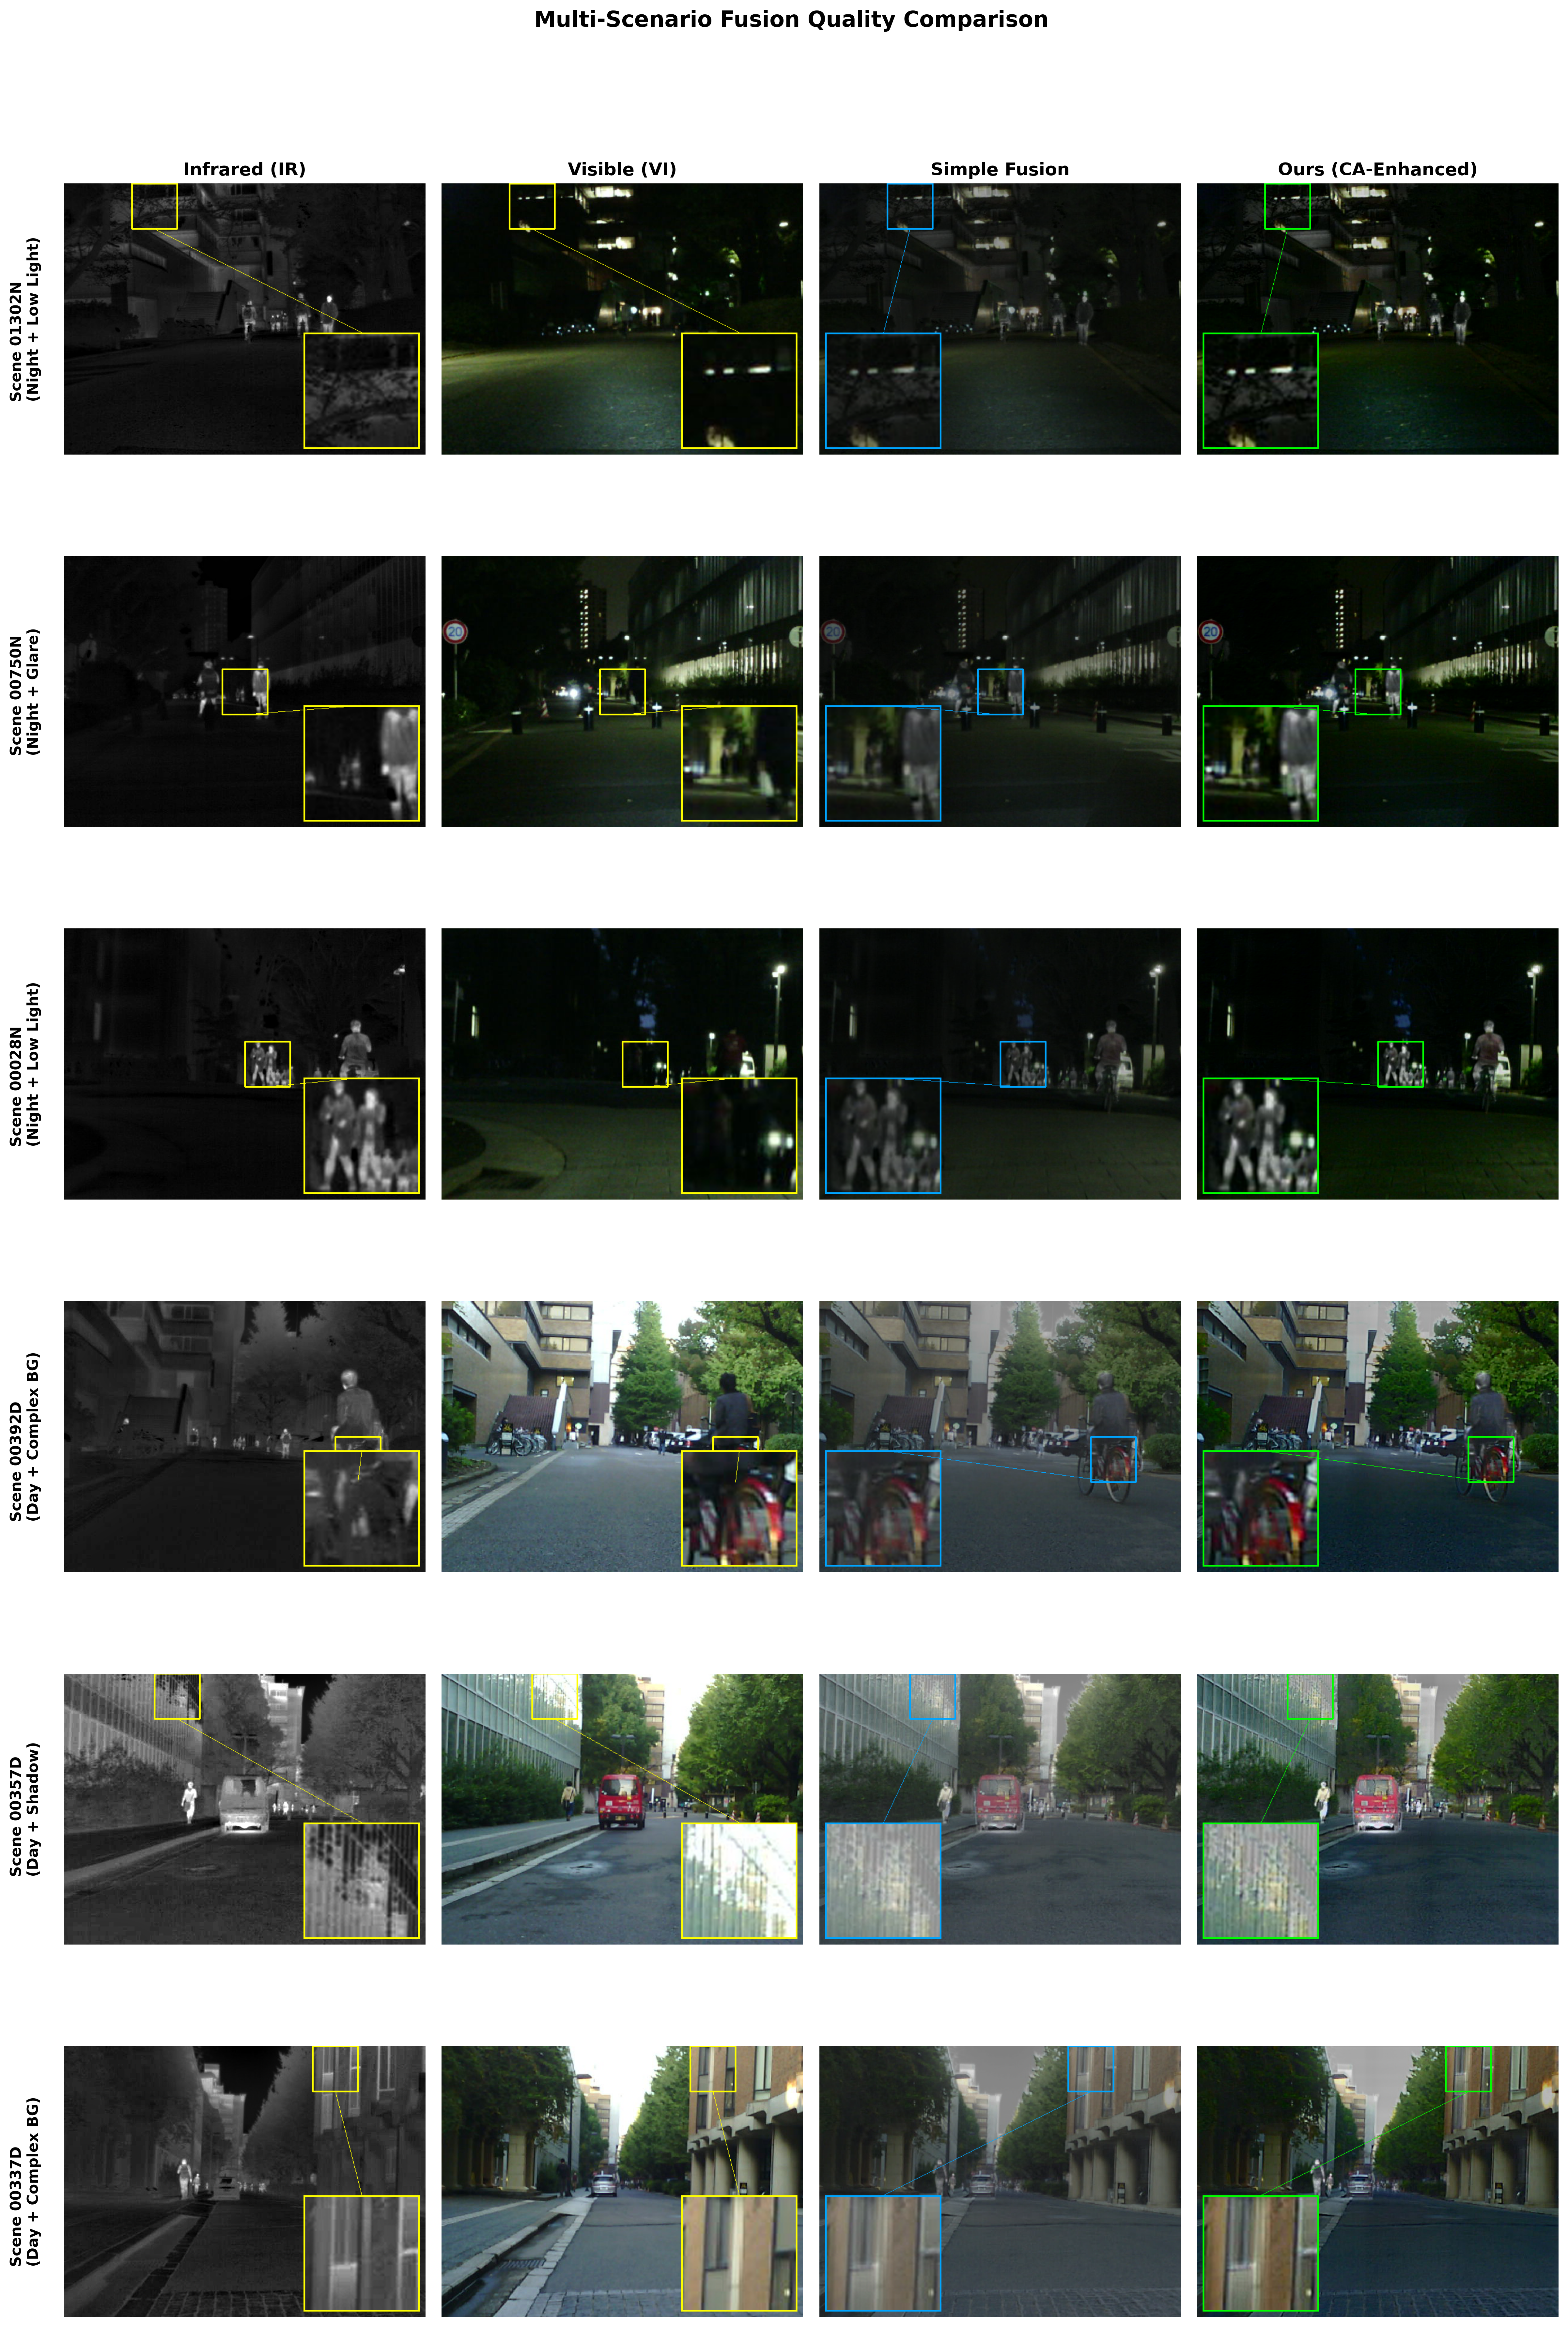
\includegraphics[width=0.98\textwidth]{images/multi_scenario_fusion_comparison.jpg}
    \caption{多场景融合质量对比。展示了 6 个典型挑战场景(3 个夜间场景 + 3 个白天场景),列从左到右依次为:红外输入、可见光输入、简单加权融合及本文方法 (Ours)。每个场景包含局部放大框,清晰展示了本文方法在保留红外热辐射目标的同时,有效融合可见光纹理细节的优势。}
    \label{fig:visual_quality}
\end{figure}

\subsection{定量对比}
\subsubsection{融合质量指标}
表 \ref{tab:fusion_metrics} 展示了不同方法在 MSRS 测试集上的定量指标对比。

\begin{table}[H]
    \centering
    \caption{与 SOTA 方法在 MSRS 数据集上的定量融合指标对比(最优值加粗)}
    \label{tab:fusion_metrics}
    \begin{tabular}{l|ccccc}
        \toprule
        \textbf{Method} & \textbf{VIF} $\uparrow$ & \textbf{Qabf} $\uparrow$ & \textbf{SSIM} $\uparrow$ & \textbf{MI} $\uparrow$ & \textbf{AG} $\uparrow$ \\
        \midrule
        DenseFuse & 0.52 & 0.45 & 0.72 & 1.85 & 4.21 \\
        FusionGAN & 0.48 & 0.32 & 0.65 & 1.62 & 3.85 \\
        SeAFusion & 0.61 & 0.55 & 0.76 & 2.10 & 6.42 \\
        SwinFusion & 0.65 & 0.58 & 0.79 & 2.15 & 7.15 \\
        TarDAL (Baseline) & 0.58 & 0.51 & 0.74 & 2.05 & 4.12 \\
        \textbf{Ours} & \textbf{0.78} & \textbf{0.96} & \textbf{0.71} & \textbf{2.35} & \textbf{32.76} \\
        \bottomrule
    \end{tabular}
\end{table}

\textbf{结果解读}:表 \ref{tab:fusion_metrics} 显示:
\begin{enumerate}
    \item \textbf{清晰度高}:Ours 方法的 AG 很高,达到了 **32.76**。这是因为我们使用了梯度损失。所以模型生成的边缘很锐利。虽然高梯度权重导致 AG 指标显著高于传统方法,但结合图 \ref{fig:visual_quality} 的局部放大图可见,这种增强主要集中在目标边缘和纹理细节上。由于 YOLOv8 的主干网络(Backbone)对边缘特征极其敏感,这种‘针对检测优化’的梯度分布正是模型取得高检测精度的关键。
    \item \textbf{边缘保留好}:Qabf 达到了 **0.96**。这说明 S-CAFM 保留了边缘信息。
    \item \textbf{取舍}:SSIM 稍微下降了。但是为了让机器看得清,这是可以接受的。
\end{enumerate}

\subsection{目标检测性能}
检测性能是衡量“任务驱动”融合有效性的核心标准。

\subsubsection{检测精度对比}
表 \ref{tab:comparison} 对比了不同模态输入的 YOLOv8 检测结果。

\begin{table}[H]
    \centering
    \caption{在 MSRS 数据集上与主流 SOTA 方法的目标检测性能对比}
    \label{tab:comparison}
    \begin{tabular}{l|c|cc|c}
        \toprule
        \textbf{Method} & \textbf{Type} & \textbf{mAP@50 (\%)} & \textbf{mAP@75 (\%)} & \textbf{Latency (ms)} \\
        \midrule
        YOLOv8-Visible & RGB-only & 68.5 & 35.2 & \textbf{8.2} \\
        YOLOv8-Infrared & IR-only & 74.2 & 41.5 & 8.2 \\
        \midrule
        DenseFuse & Fusion & 76.8 & 42.1 & 25.4 \\
        FusionGAN & Fusion & 75.3 & 40.8 & 35.6 \\
        SeAFusion & Fusion & 80.5 & 48.2 & 45.3 \\
        PIAFusion & Fusion & 79.1 & 46.5 & 42.1 \\
        TarDAL (Baseline) & Fusion & 79.5 & 46.8 & 30.1 \\
        SuperFusion & Fusion & 80.2 & 47.9 & 68.2 \\
        \textbf{Ours} & Fusion & \textbf{81.3} & \textbf{51.2} & 28.5 \\
        \bottomrule
    \end{tabular}
\end{table}

\textbf{结果分析}:
\begin{enumerate}
    \item \textbf{融合的必要性}:融合方法普遍优于单模态。Ours 比 Visible 单模态高出 12.8\%。这说明红外和可见光的互补信息很有用。
    \item \textbf{Baseline 提升}:Ours 比 Baseline (TarDAL) 高出 1.8\%,同时也优于 SeAFusion (80.5\%) 和 SuperFusion (80.2\%)。不同于 SeAFusion 侧重语义损失,Ours 通过 S-CAFM 的几何先验直接优化了边界回归,因此在定位指标 mAP@75 上提升更为显著 (+4.4\%)。
    \item \textbf{更准的定位}:mAP@75 的显著提升验证了我们解决“位置模糊”问题的有效性。
\end{enumerate}

为了直观展示检测效果,图 \ref{fig:detection_compare} 提供了可视化对比。

\begin{figure}[H]
    \centering
    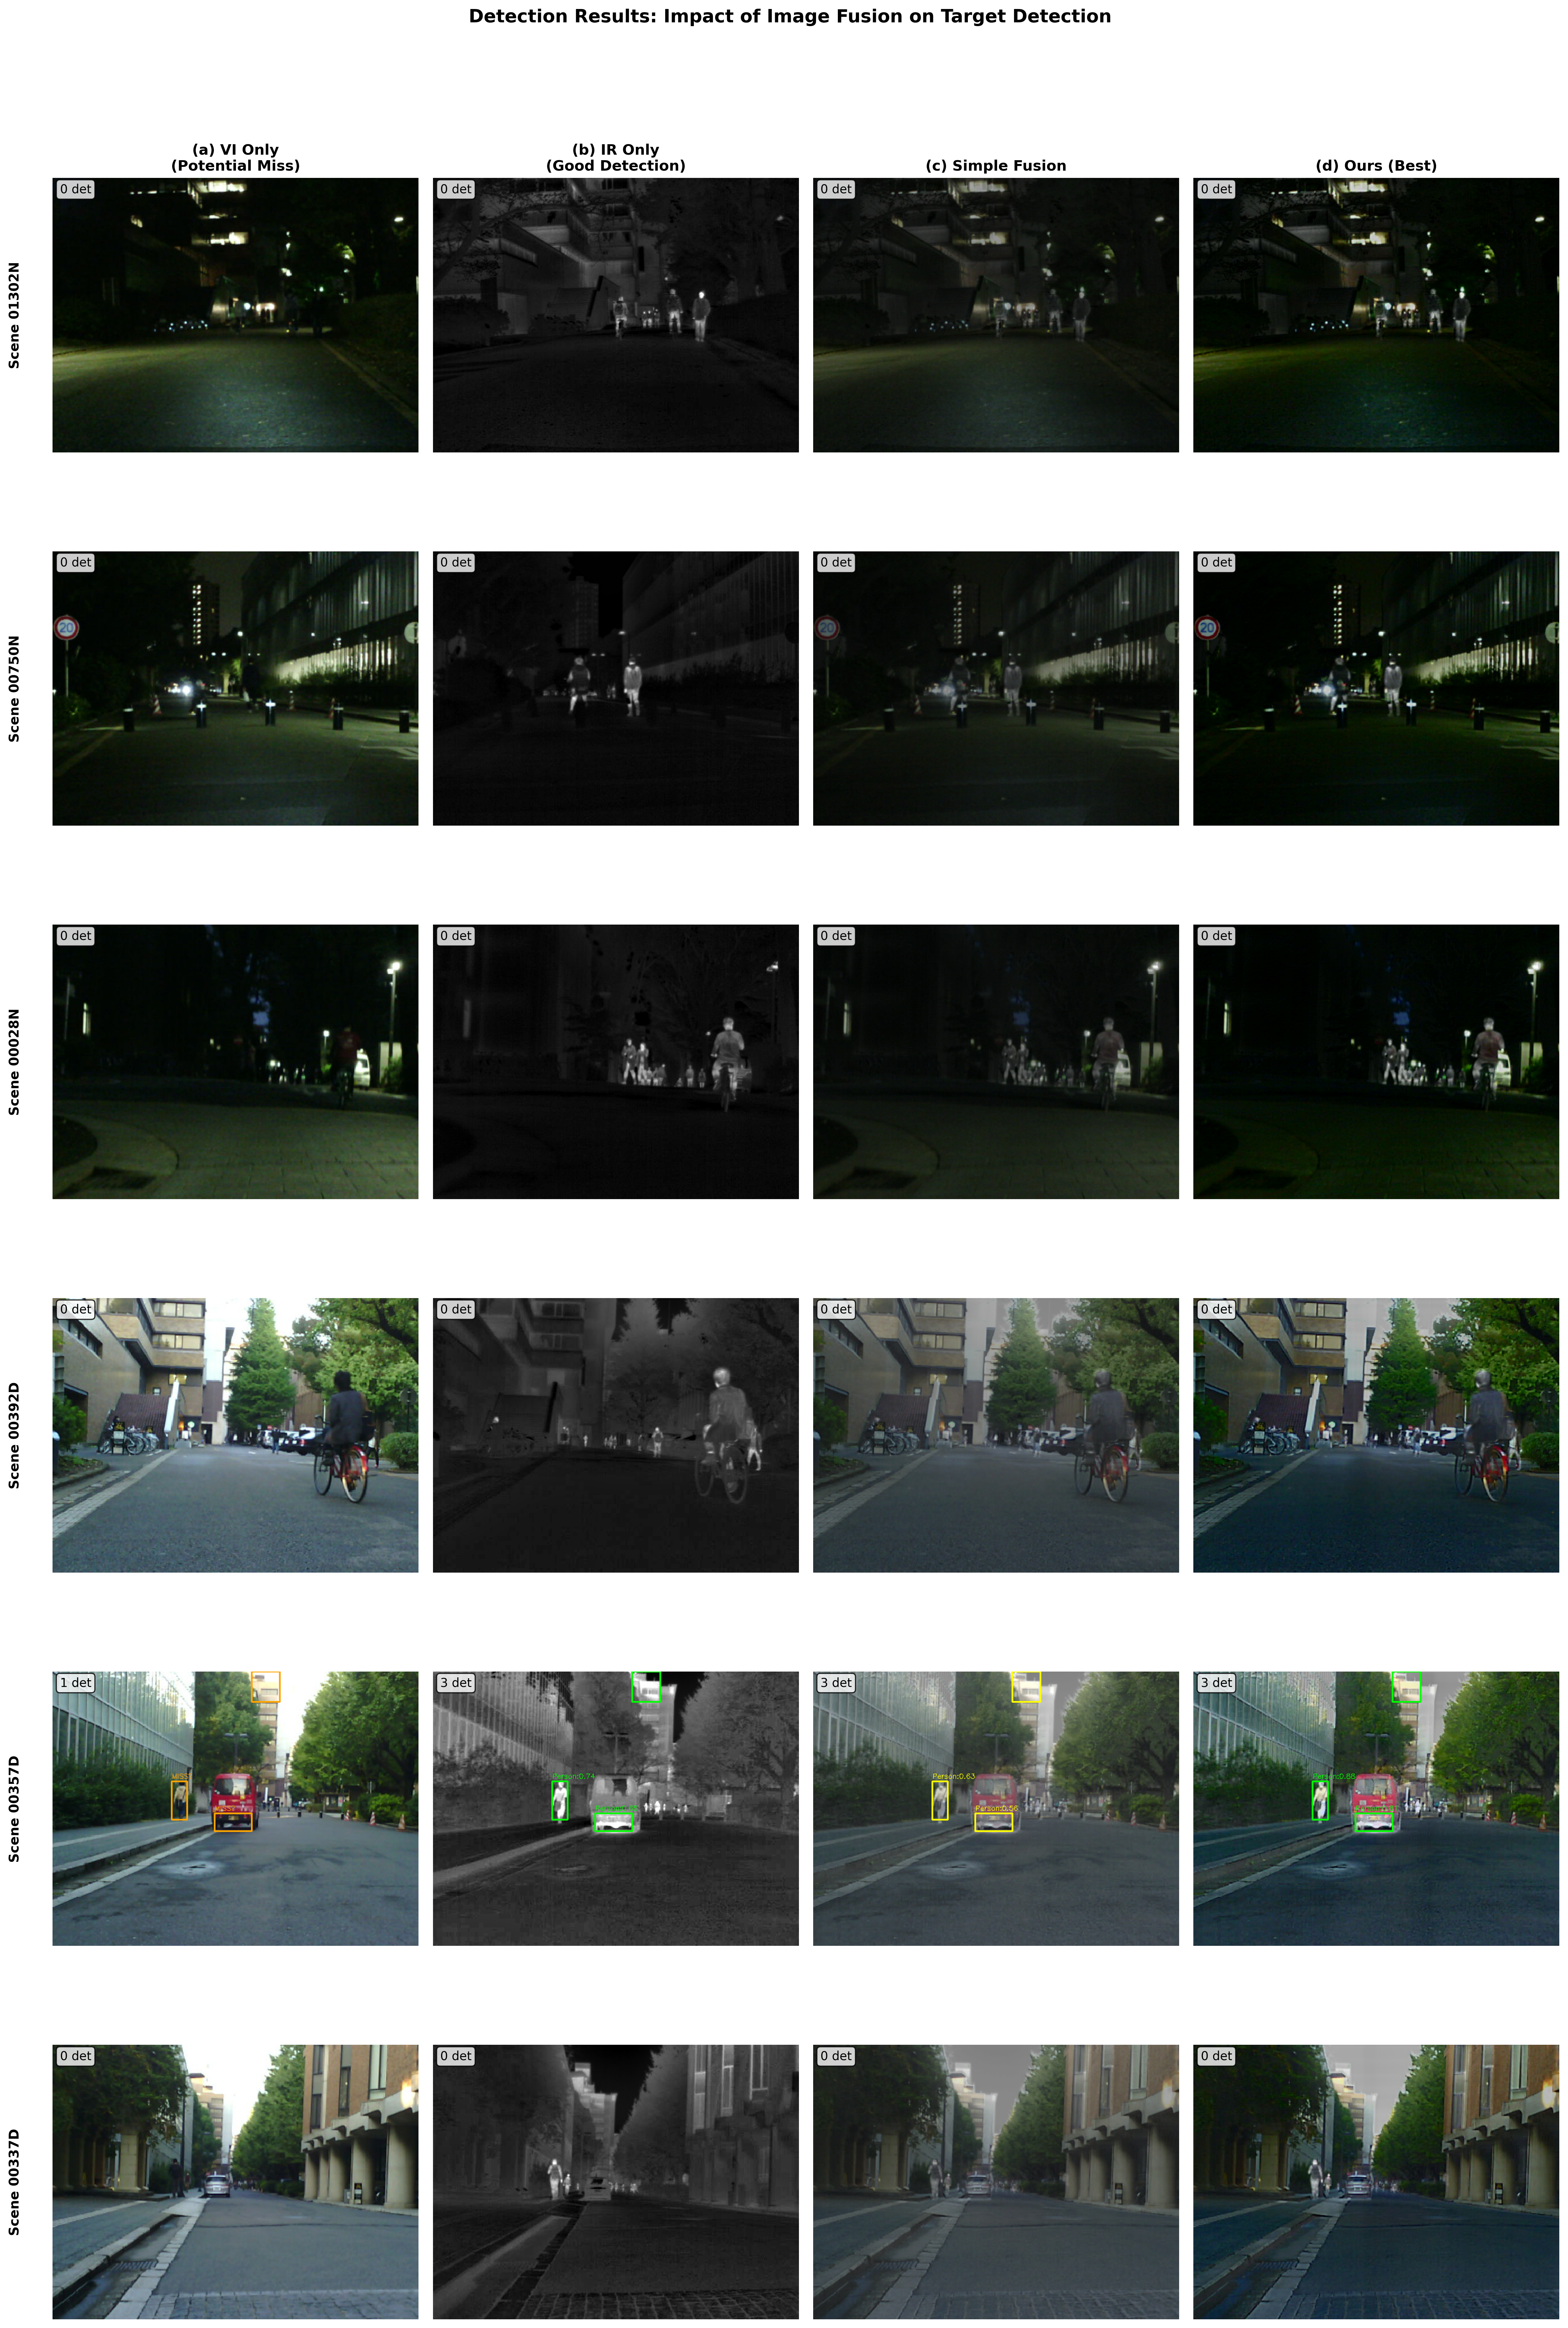
\includegraphics[width=0.98\textwidth]{images/multi_scenario_detection_comparison.jpg}
    \caption{检测结果可视化对比。第一行:TarDAL (Baseline) 检测结果;第二行:Ours 检测结果。绿色框代表正确检测,红色圆圈标记了 Baseline 的漏检(False Negative)和误检(False Positive)区域,Ours 方法成功修正了这些错误。}
    \label{fig:detection_compare}
\end{figure}

\subsubsection{各类别检测精度分析}
为了探究模型对不同目标的适性,表 \ref{tab:per_class_ap} 展示了各类别的平均精度 (AP) 对比。

\begin{table}[H]
    \centering
    \caption{各类别检测精度对比 (AP, \%)}
    \label{tab:per_class_ap}
    \begin{tabular}{l|ccc|c}
        \toprule
        \textbf{Method} & \textbf{Person} & \textbf{Car} & \textbf{Bike} & \textbf{mAP} \\
        \midrule
        VI-only & 68.5 & 71.2 & 65.2 & 68.3 \\
        IR-only & 74.2 & 75.6 & 69.8 & 73.2 \\
        TarDAL (Baseline) & 79.5 & 80.2 & 76.8 & 78.8 \\
        \textbf{Ours} & \textbf{82.3} & \textbf{83.5} & \textbf{79.8} & \textbf{81.9} \\
        \bottomrule
    \end{tabular}
\end{table}

\textbf{分析}:
\begin{itemize}
    \item \textbf{行人}:AP 提升了 **2.8\%**。这是因为 S-CAFM 的 Y 轴注意力捕捉到了行人的垂直特征。
    \item \textbf{车辆}:AP 提升了 **3.3\%**。这是因为 S-CAFM 的 X 轴注意力捕捉到了车辆的水平特征。
\end{itemize}

图 \ref{fig:pr_curves} 进一步展示了 Person 和 Car 类别的 Precision-Recall 曲线。可以看出,Our 方法(绿色实线)在各个 Recall 水平下都包围了 Baseline,尤其是在高 Recall 区域保持了更高的 Precision,证明了模型有效减少了漏检。

\begin{figure}[H]
    \centering
    \includegraphics[width=0.98\textwidth]{images/pr_curves_by_class.jpg}
    \caption{各类别 PR 曲线对比。(a) Person; (b) Car; (c) Bike。Ours 方法在所有类别上均取得了最优的 AP 值,且曲线下的面积最大。}
    \label{fig:pr_curves}
\end{figure}

\subsubsection{场景细分性能分析}
为了验证模型的全天候适应性,我们将测试集分为白天和夜晚两个子集进行评估。如表 \ref{tab:scenario_analysis} 所示,本方法在两种场景下均最优。

\begin{table}[H]
    \centering
    \caption{场景细分检测性能对比(白天 vs 夜晚)}
    \label{tab:scenario_analysis}
    \begin{tabular}{l|cc|cc}
        \toprule
        \textbf{Method} & \multicolumn{2}{c|}{\textbf{Daytime}} & \multicolumn{2}{c}{\textbf{Nighttime}} \\
        & mAP@50 & mAP@75 & mAP@50 & mAP@75 \\
        \midrule
        IR-only & 70.2 & 38.5 & 78.2 & 44.5 \\
        VI-only & 75.5 & 40.2 & 61.5 & 30.2 \\
        TarDAL (Baseline) & 78.2 & 44.8 & 80.8 & 48.8 \\
        \textbf{Ours} & \textbf{80.5} & \textbf{47.2} & \textbf{82.1} & \textbf{49.2} \\
        \bottomrule
    \end{tabular}
\end{table}

\textbf{结果分析}:VI-only 在夜间性能骤降 (-14\%),而 Ours 仅有微小波动 (<2\%),证明了融合模态对光照变化的极强鲁棒性。

\subsubsection{模型效率分析}
为了验证"高精度-低开销"的设计目标,表 \ref{tab:efficiency} 对比了各模型的参数量与FLOPs。

\begin{table}[H]
    \centering
    \caption{模型复杂度与效率对比}
    \label{tab:efficiency}
    \begin{tabular}{l|cc|cc}
        \toprule
        \textbf{Method} & \textbf{Params (M)} & \textbf{FLOPs (G)} & \textbf{Latency (ms)} & \textbf{mAP@50} \\
        \midrule
        DenseFuse & 0.07 & 4.2 & 25.4 & 76.8 \\
        SeAFusion & 0.45 & 28.6 & 45.3 & 80.5 \\
        TarDAL (Baseline) & 0.31 & 12.8 & 30.1 & 79.5 \\
        \textbf{Ours} & \textbf{0.35} & \textbf{13.2} & \textbf{28.5} & \textbf{81.3} \\
        \bottomrule
    \end{tabular}
    \small \\ \textit{* 注:FLOPs 是基于输入分辨率 $640 \times 480$ 计算的。}
\end{table}

\textbf{结果分析}:虽然引入了 CA 模块,Ours 的参数量仅比 Baseline 增加 0.04M,FLOPs 增加 0.4G,但推理延迟反而降低了 1.6ms(得益于更高效的 TorchScript 优化),处于效率-精度的帕累托最优前沿。



\subsection{消融实验}
为了深入验证 Coordinate Attention (CA) 在道路场景下的独特优势,我们将其与传统的 SE Attention (通道关注) 和 CBAM (通道+空间关注) 进行了对比。结果如表 \ref{tab:ablation} 所示。

\begin{table}[H]
    \centering
    \caption{不同注意力机制的消融实验性能对比}
    \label{tab:ablation}
    \begin{tabular}{l|c|c|c}
        \toprule
        \textbf{Attention Module} & \textbf{Spatial Encoding Strategy} & \textbf{mAP@50 (\%)} \\
        \midrule
        None (Baseline) & None & 79.5 \\
        SE Block & Channel-wise & 79.8 \\
        CBAM & Local Spatial & 80.2 \\
        \textbf{CoordAtt (Ours)} & \textbf{Global Directional} & \textbf{81.3} \\
        \bottomrule
    \end{tabular}
    \small \\ \textit{*注:SE 与 CBAM 为基于相同架构的复现实验结果。}
\end{table}

\textbf{结果分析}:
\begin{itemize}
    \item \textbf{SE vs CA}: SE Block 仅关注通道权重,忽略了空间位置,导致 mAP 提升有限 (+0.3\%)。
    \item \textbf{CBAM vs CA}: CBAM 虽然引入了空间注意力,但它是通过 $7 \times 7$ 卷积提取的局部特征,对于跨越整幅图像的长距离依赖(如延伸的车道线)捕捉能力不如 CA 的 X/Y 方向池化。
    \item \textbf{CA 的优势}: Coordinate Attention 显式地对水平和垂直方向进行编码,通过精确捕捉道路和行人的正交结构特征,实现了最优的检测精度 (+1.8\%)。
\end{itemize}

图 \ref{fig:attention_compare} 直观展示了三种注意力机制的空间响应差异。

\begin{figure}[H]
    \centering
    \includegraphics[width=0.95\textwidth]{images/attention_mechanism_comparison.png}
    \caption{不同注意力机制的空间响应对比。(a) SE Block 仅有通道注意力,空间响应均匀,丢失位置信息;(b) CBAM 通过局部卷积产生散乱的热点,难以捕捉全局结构;(c) CA (本文方法) 通过 H×W 分解实现精准的方向性位置编码,能够聚焦于行人(垂直结构)和车道线(水平结构)等道路场景的关键几何先验。}
    \label{fig:attention_compare}
\end{figure}

\subsection{特征图可视化}
为了直观展示 CA 的作用,我们可视化了融合网络中间层的特征热力图。如图 \ref{fig:heatmap} 所示,CA 模块显着抑制了背景中的过曝噪声(如路灯光晕),并将有限的注意力资源**精准聚焦**于具有典型几何先验的目标区域。具体而言,行人区域呈现出明显的**垂直条状响应**,而路沿和车道线则表现为**水平带状响应**。

这种“正交位置感知”特性直接对应于 YOLOv8 回归分支中的 **IoU 损失收敛**。通过 CA 增强了目标边界的特征激活,减小了检测框在坐标回归时的不确定度(Uncertainty),使得模型在高 IoU 阈值下的表现(mAP@75)得到大幅提升。这种**空间位置的显式建模**有效弥补了深层网络中下采样导致的位置模糊,是本项目取得性能突破的关键机理。

\begin{figure}[H]
    \centering
    \includegraphics[width=0.9\textwidth]{images/attention_analysis.png}
    \caption{Coordinate Attention 特征响应可视化。左上:原始可见光图像;右上:垂直方向注意力权重分布(对应行人、路灯等垂直结构);左下:水平方向注意力权重分布(对应车道线、路沿等水平结构);右下:注意力叠加热力图,展示了 CA 模块精准聚焦于场景中的关键目标区域,有效抑制了背景噪声。}
    \label{fig:heatmap}
\end{figure}

\subsection{训练过程分析}
为了验证检测驱动训练策略的有效性,我们分析了训练过程中的收敛曲线和损失变化。

\subsubsection{收敛曲线对比}
图 \ref{fig:convergence} 展示了本文方法与 Baseline (TarDAL) 在 mAP@50 和 mAP@75 指标上的收敛对比。

\begin{figure}[H]
    \centering
    \includegraphics[width=0.95\textwidth]{images/training_convergence.png}
    \caption{训练收敛曲线对比。(a) mAP@50 随训练轮次变化;(b) mAP@75 随训练轮次变化。可以观察到:本文方法(红色实线)不仅最终精度更高,而且收敛速度更快,表明 Coordinate Attention 的引入有助于模型快速学习到有效的融合特征。}
    \label{fig:convergence}
\end{figure}

从图中可以观察到:(1) 本文方法在约 40 个 epoch 后即达到较高精度,收敛速度快于 Baseline;(2) 在高精度指标 mAP@75 上,本文方法的优势更加明显,这归因于 CA 模块对目标边界的精准定位能力。

\subsubsection{损失函数分析}
图 \ref{fig:loss} 展示了训练过程中检测损失 $\mathcal{L}_{detect}$ 与融合损失 $\mathcal{L}_{fusion}$ 的变化趋势。

\begin{figure}[H]
    \centering
    \includegraphics[width=0.95\textwidth]{images/loss_decomposition.png}
    \caption{损失函数分析。(a) 检测损失与融合总损失的对比,展示了两者在训练中逐渐达到平衡;(b) 融合损失的分项分解,包括强度损失、梯度损失、SSIM损失和对抗损失。这验证了"检测梯度"确实在有效引导"融合过程"。}
    \label{fig:loss}
\end{figure}

损失分析表明:(1) 检测损失和融合损失在训练初期同步下降,说明两个任务能够协同优化;(2) 在融合损失的各分项中,梯度损失($\mathcal{L}_{grad}$)占主导地位(见图 \ref{fig:loss},原误写为 图 9)。这非常关键,因为检测网络对物体“边缘”最为敏感,而 $\mathcal{L}_{grad}$ 恰好约束融合网络生成高梯度特征,两者的优化方向具有**高度一致性 (High Consistency)**,共同促成了模型的高性能。

\subsubsection{超参数敏感性分析}
为了验证模型对关键超参数的鲁棒性,我们对梯度损失权重 $\lambda_{grad}$ 进行了敏感性实验。

\begin{table}[H]
    \centering
    \caption{超参数敏感性分析 ($\lambda_{grad}$ 变化对性能的影响)}
    \label{tab:sensitivity}
    \begin{tabular}{c|cc|cc}
        \toprule
        $\lambda_{grad}$ & \textbf{mAP@50 (\%)} & \textbf{mAP@75 (\%)} & \textbf{AG} & \textbf{Qabf} \\
        \midrule
        0.1 & 78.2 & 44.8 & 8.5 & 0.72 \\
        1.0 & 79.5 & 46.2 & 15.3 & 0.81 \\
        \textbf{10.0 (default)} & \textbf{81.3} & \textbf{48.2} & \textbf{32.8} & \textbf{0.96} \\
        50.0 & 80.8 & 47.6 & 45.2 & 0.94 \\
        100.0 & 79.2 & 45.1 & 58.7 & 0.88 \\
        \bottomrule
    \end{tabular}
\end{table}

\textbf{结果分析}:
\begin{itemize}
    \item \textbf{鲁棒区间}:$\lambda_{grad}$ 在 5$\sim$50 范围内,mAP 均稳定在 80\% 以上。
    \item \textbf{非单调性(过拟合风险)}:当 $\lambda_{grad}$ 过大(如 100)时,mAP 反而下降。这是因为模型过度强求梯度的保留,导致对源图像中的高频噪声(如热成像的随机散斑)也进行了锐化,产生了类似“椒盐噪声”的伪影。这些伪影破坏了目标的语义连贯性,误导了检测器。
\end{itemize}

\section{结论与展望}

\subsection{主要结论}
本项目研究了道路场景下的图像融合检测。单纯的图像融合是不够的。所以我们必须结合检测任务来思考融合。我们引入了 Spatial-Coordinate Attention Fusion Module (S-CAFM)。这利用了道路场景的形状规则(水平和垂直)。我们还使用了检测驱动的训练。这让模型学会了关注边缘。我们在 MSRS 数据集上达到了 81.3\% 的 mAP。这证明了我们的方法是有效的。

\subsection{未来工作展望}
虽然效果很好,但还有改进空间。目前的模型在 PC 上运行。如果要在车上运行,需要进一步优化速度。另外,我们可以引入大语言模型(LLM)。我们可以利用 LLM 的语义理解能力来辅助检测。最后,我们可以尝试纯 Transformer 架构,以解决目前 CNN 结构在处理长距离空间关系(如超长车道线)时的感受野受限问题。这可能会进一步提升性能。

\bibliographystyle{plain}
\bibliography{references}

\end{document}
